\frame
{
\frametitle{Introduction}

The bootstrap method is not always the best one. One main reason is that the bootstrap samples are generated from $\hat{f}$ and not from $f$. \alert{Can we find samples/resamples exactly generated from $f$?}

\begin{itemize}
\item If we look for samples of size $n$, then the answer is \alert{no}!
\item If we look for samples of size $m$ ($m<n$), then we can indeed find (re)samples of size $m$ exactly generated from $f$ simply by looking at different subsets of our original sample $\mathbf{x}$! 
\end{itemize}

Looking at different subsets of our original sample amounts to sampling without replacement from observations $x_1,\cdots,x_n$ to get (re)samples (now called \alert{subsamples}) of size $m$. This leads us to subsampling and the jackknife.  
}

\frame
{
\frametitle{Jackknife}

\begin{itemize}
\item  The jackknife has been proposed by Quenouille in mid 1950's.

\

\item In fact, the jackknife predates the bootstrap. 

\

\item The jackknife (with $m=n-1$) is less computer-intensive than the bootstrap. 

\

\item \textit{Jackknife} describes a swiss penknife, easy to carry around. By analogy, Tukey (1958) coined the term in statistics as a general approach for testing hypotheses and calculating confidence intervals.  


\end{itemize}

}
%%%%%%%%%%%%%%%%%%%%%%%%%%%%%%%%%%%%%%%%%%%%%%%%%%%
\frame
{
\frametitle{Jackknife samples}

\begin{definition}
The \alert{Jackknife samples} are computed by leaving out one observation $x_i$ from $\mathbf{x}=(x_{1},x_{2},\cdots,x_{n})$ at a time:
$$
\mathbf{x}_{(i)}=(x_{1},x_{2},\cdots,x_{i-1},x_{i+1},\cdots,x_{n})
$$ 
\end{definition}

\begin{beamercolorbox}[wd=\linewidth, rounded=true,shadow=true]{postit}
\begin{itemize}
\item The dimension of the jackknife sample $\mathbf{x}_{(i)}$ is $m=n-1$  
\item $n$  different Jackknife samples :  $\lbrace\mathbf{x}_{(i)}\rbrace_{i=1\cdots n}$.
\item No sampling method needed to compute the $n$  jackknife samples.

\end{itemize}
\end{beamercolorbox}
\begin{block}{}
\tiny{Available BOOTSTRAP MATLAB TOOLBOX, by Abdelhak M. Zoubir and D. Robert Iskander, 
\href{http://www.csp.curtin.edu.au/downloads/bootstrap_toolbox.html}{http://www.csp.curtin.edu.au/downloads/bootstrap\_toolbox.html}}
\end{block}
}

%%%%%%%%%%%%%%%%%%%%%%%%%%%%%%%%%%%%%%%%%%%%%%%%%%%%%%
\frame
{
\frametitle{Jackknife replications}

\begin{definition}
The ith \alert{jackknife replication} $\hat{\theta}_{(i)}$ of the statistic $\hat{\theta}=s(\mathbf{x})$ is:
$$ 
\hat{\theta}_{(i)}=s(\mathbf{x}_{(i)}),\quad \forall i=1,\cdots,n
$$
\end{definition}

\begin{exampleblock}{Jackknife replication of the mean}


$$
\begin{array}{ll}
s(\mathbf{x}_{(i)})&=\frac{1}{n-1}\sum_{j\neq i } x_j\\
&\\
&=\frac{(n\overline{x}-x_i)}{n-1} \\
&\\
&=\overline{x}_{(i)}\\
\end{array}
$$

\end{exampleblock}
}
%%%%%%%%%%%%%%%%%%%%%%%%%%%%%%%%%%%%%%%%%%%%%%%%%%%%
\frame
{
\frametitle{Jackknife estimation of the standard error}


\begin{beamercolorbox}[wd=\linewidth, rounded=true,shadow=true]{postit}

\begin{enumerate}
\item Compute the $n$ jackknife subsamples $\mathbf{x}_{(1)}, \cdots,\mathbf{x}_{(n)}$ from $\mathbf{x}$.

\

\item Evaluate the $n$ jackknife replications $\hat{\theta}_{(i)}=s(\mathbf{x}_{(i)})$.

\

\item The \alert{jackknife estimate of the standard error} is defined by:
$$
\hat{\mathrm{se}}_{jack}=\left \lbrack \frac{n-1}{n} \sum_{i=1}^{n} (\hat{\theta}_{(\cdot)}-\hat{\theta}_{(i)})^{2}\right\rbrack^{1/2}
$$
where $\hat{\theta}_{(\cdot)}=\frac{1}{n}\sum_{i=1}^{n} \hat{\theta}_{(i)}$.

\end{enumerate}
\end{beamercolorbox}
}
%%%%%%%%%%%%%%%%%%%%%%%%%%%%%%%%%%%%%%%%%%%%%%%%%%%%
\frame
{
\frametitle{Jackknife estimation of the standard error of the mean}

For $\hat{\theta}=\overline{x}$, it is easy to show that: 
$$
\left\lbrace
\begin{array}{l}
\overline{x}_{(i)}=\frac{n\overline{x}-x_i}{n-1}\\
\\
\overline{x}(\cdot)=\frac{1}{n}\sum_{i=1}^{n} \overline{x}_{(i)}=\overline{x}\\
\end{array}
\right.
$$
 Therefore:
$$
\begin{array}{ll}
\widehat{\mathrm{se}}_{jack}&=\left\lbrace \sum_{i=1}^n \frac{(x_i-\overline{x})^2}{(n-1)n} \right\rbrace^{1/2}\\
&\\
& =  \frac{\overline{\sigma}}{\sqrt{n}}\\
\end{array}
$$
where $\overline{\sigma}$ is the unbiased variance. 

}
%%%%%%%%%%%%%%%%%%%%%%%%%%%%%%%%%%%%%%%%%%%%%%%%%%%%
\frame
{
\frametitle{Jackknife estimation of the standard error}

\begin{itemize}
\item The factor $\frac{n-1}{n}$ is much larger than $\frac{1}{B-1}$ used in bootstrap. 

\

\item Intuitively this inflation factor is needed because jackknife deviation $(\hat{\theta}_{(i)}-\hat{\theta}_{(\cdot)})^{2}$ tend to be smaller than the bootstrap  $(\hat{\theta}^{*}(b)-\hat{\theta}^{*}(\cdot))^{2}$ (the jackknife sample is more similar to the original data $\mathbf{x}$ than the bootstrap).  

\

\item In fact, the factor $\frac{n-1}{n}$ is derived by considering the special case $\hat{\theta}=\overline{x}$ (somewhat arbitrary convention).  
\end{itemize}
}
%%%%%%%%%%%%%%%%%%%%%%%%%%%%%%%%%%%%%%%%%%%%%%%%%%%%
\frame
{
\frametitle{Comparison of Jackknife and Bootstrap on an example}
\begin{exampleblock}{Example A: $\hat{\theta}=\overline{x}$}
%We consider $\hat{\theta}=\overline{x}$ computed over an observation $\mathbf{x}$ of $n=100$ values sampled from the distribution: 
 $f(x)=0.2\ \mathcal{N}(\scriptstyle \mu=1,\sigma=2 \displaystyle) +0.8\  \mathcal{N}( \scriptstyle\mu=6,\sigma=1 \displaystyle)
$   $\rightsquigarrow\mathbf{x}=(x_1,\cdots,x_{100})$. 
\begin{itemize}
\item  Bootstrap standard error and bias w.r.t. the number $B$ of bootstrap samples: 
\end{itemize}
%\begin{table}[!h]
\begin{tabular}{|c|c|c|c|c|c|c|c|}
\hline
$B$& 10& 20 & 50 & 100 & 500 & 1000  & 10000\\
\hline
$\widehat{\mathrm{se}}_{B}$& \small{0.1386} & \small{0.2188} & \small{0.2245} & \small{0.2142} & \small{0.2248}& \small{0.2212} & \small{0.2187}\\
\hline
$\widehat{\mathrm{Bias}}_{B}$ & \small{0.0617} & \small{-0.0419} & \small{0.0274} & \small{-0.0087} & \small{-0.0025} &  \small{0.0064} & \small{0.0025} \\
%\small{-0.1062} & \small{-0.0532} & \small{-0.0364} &  \small{-0.0199} & \small{-0.0003} & \small{-0.001} & \small{-0.002}\\
\hline
\end{tabular}

\

%\caption{\small{Bootstrap standard error and bias w.r.t. the number $B$ of bootstrap samples.}}
%\end{table}
\begin{itemize}
\item Jackknife: $\widehat{\mathrm{se}}_{jack}=0.2207$ and  $\widehat{\mathrm{Bias}}_{jack}= 0$

\

\item Using textbook formulas:  $ \mathrm{se}_{\hat{f}}=\frac{\hat{\sigma}}{\sqrt{n}}=0.2196$  ($\frac{\overline{\sigma}}{\sqrt{n}}=0.2207$).
\end{itemize}
\end{exampleblock}

}

%%%%%%%%%%%%%%%%%%%%%%%%%%%%%%%%%%%%%%%%%%%%%%%%%%%%
\frame
{
\frametitle{Jackknife estimation of the bias}


\begin{beamercolorbox}[wd=\linewidth, rounded=true,shadow=true]{postit}
\begin{enumerate}
\item Compute the $n$ jackknife subsamples $\mathbf{x}_{(1)}, \cdots,\mathbf{x}_{(n)}$ from $\mathbf{x}$.

\

\item Evaluate the $n$ jackknife replications $\hat{\theta}_{(i)}=s(\mathbf{x}_{(i)})$.

\

\item The \alert{jackknife estimation of the bias} is defined as:
$$
\widehat{\mathrm{Bias}}_{jack}=(n-1)(\hat{\theta}_{(\cdot)}-\hat{\theta})
$$
where $\hat{\theta}_{(\cdot)}=\frac{1}{n}\sum_{i=1}^{n} \hat{\theta}_{(i)}$. 

\end{enumerate}
%This formula applies only to plug-in statistics $\hat{\theta}=t(\hat{F})$.

\end{beamercolorbox}
}
%%%%%%%%%%%%%%%%%%%%%%%%%%%%%%%%%%%%%%%%%%%%%%%%%%%%
\frame
{
\frametitle{Jackknife estimation of the bias}

\begin{itemize}
\item Note the inflation factor $(n-1)$ (compared to the bootstrap bias estimate).

\

\item $\hat{\theta}=\overline{x}$ is unbiased so the correspondence is done considering the plug-in estimate of the variance $\hat{\sigma}^2=\frac{\sum_{i=1}^n (x_i-\overline{x})^2}{n}$. 

\

\item The jackknife estimate of the bias for the plug-in estimate of the variance is then:
$$    
\widehat{\mathrm{Bias}}_{jack}=\frac{\overline{-\sigma}^2}{n}
$$
\end{itemize}
}
%%%%%%%%%%%%%%%%%%%%%%%%%%%%%%%%%%%%%%%%%%%%%%%%%%%%
\frame
{
\frametitle{Histogram of the replications} 

\begin{exampleblock}{Example A}
\begin{figure}[!h]
\begin{tabular}{p{5cm}p{5cm}}
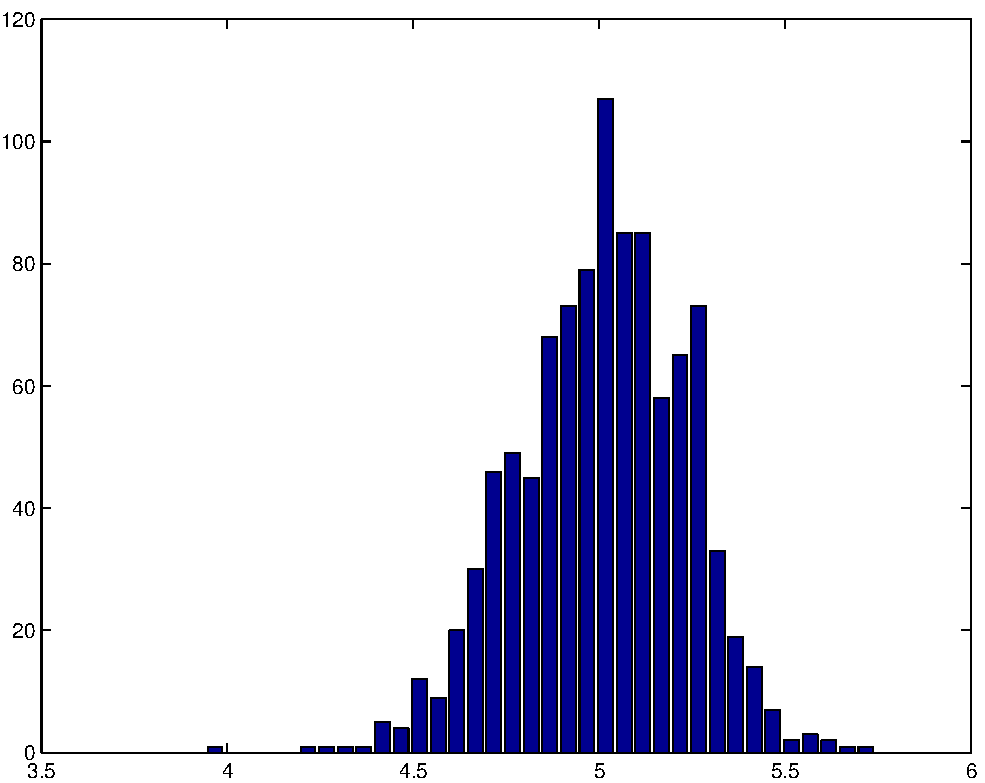
\includegraphics[width=5cm]{histobootreplications}&
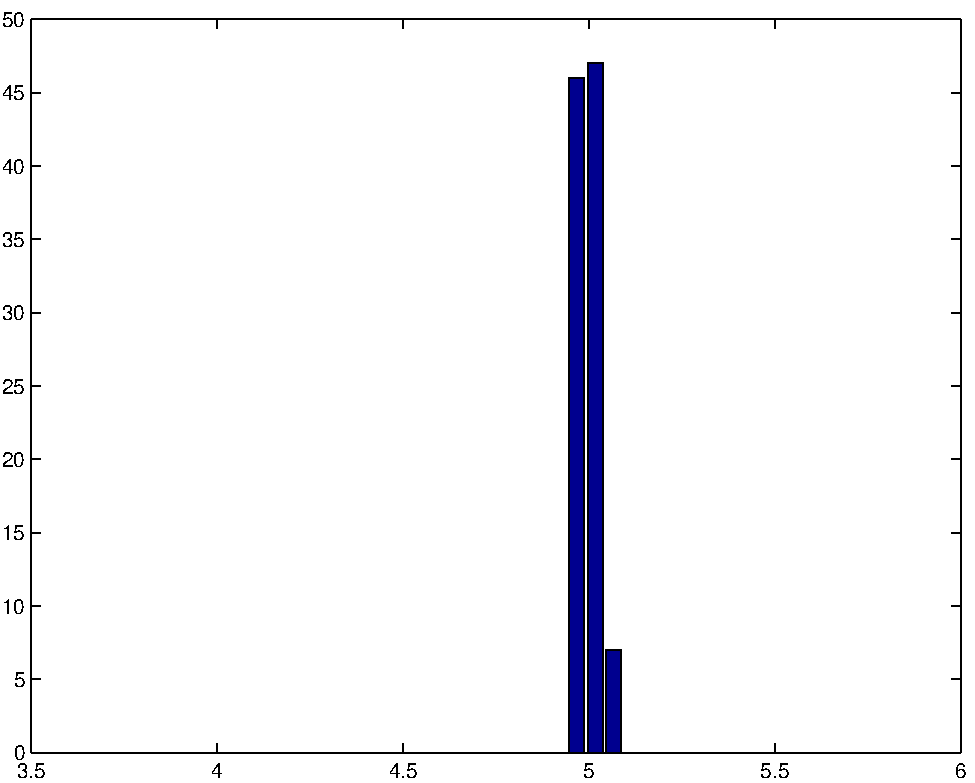
\includegraphics[width=5cm]{histojackreplications}\\
\end{tabular}
\caption{Histograms of the bootstrap replications $\lbrace \hat{\theta}^{*}(b)\rbrace_{b\in \lbrace 1,\cdots,B=1000 \rbrace}$ (left), and the jackknife replications $\lbrace \hat{\theta}_(i)\rbrace_{i\in \lbrace 1,\cdots,n=100 \rbrace}$ (right).}
\end{figure}
\end{exampleblock}
}
%%%%%%%%%%%%%%%%%%%%%%%%%%%%%%%%%%%%%%%%%%%%%%%%%%%%
\frame
{
\frametitle{Histogram of the replications} 
\begin{exampleblock}{Example A}
\begin{figure}[!h]
\begin{tabular}{p{5cm}p{5cm}}
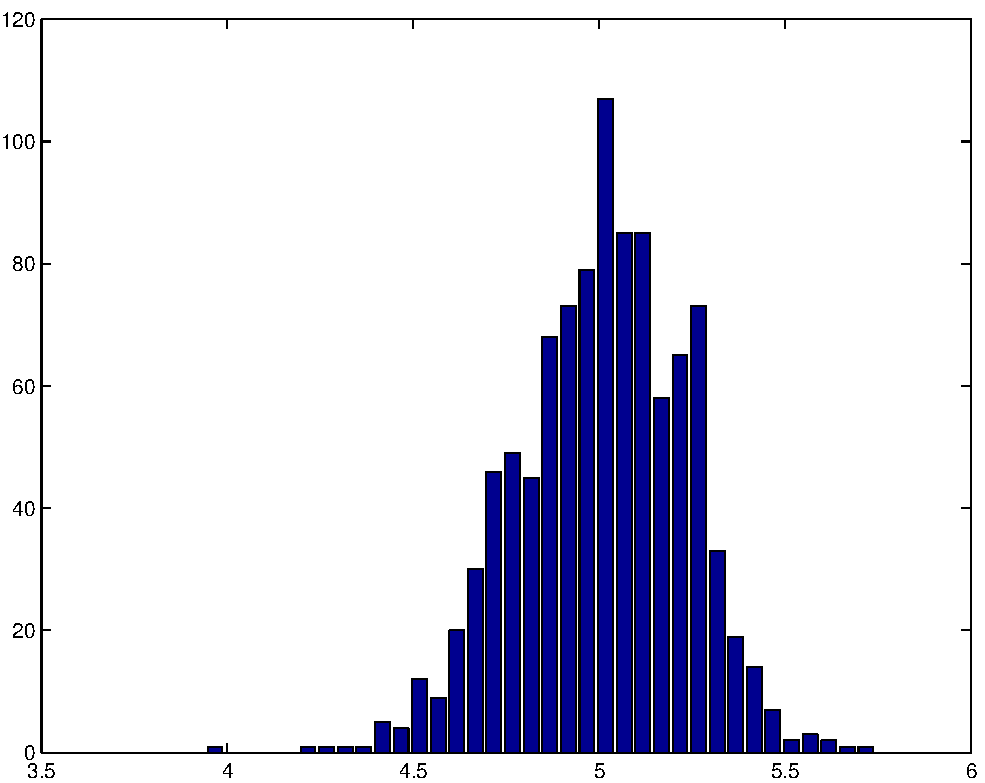
\includegraphics[width=5cm]{histobootreplications}&
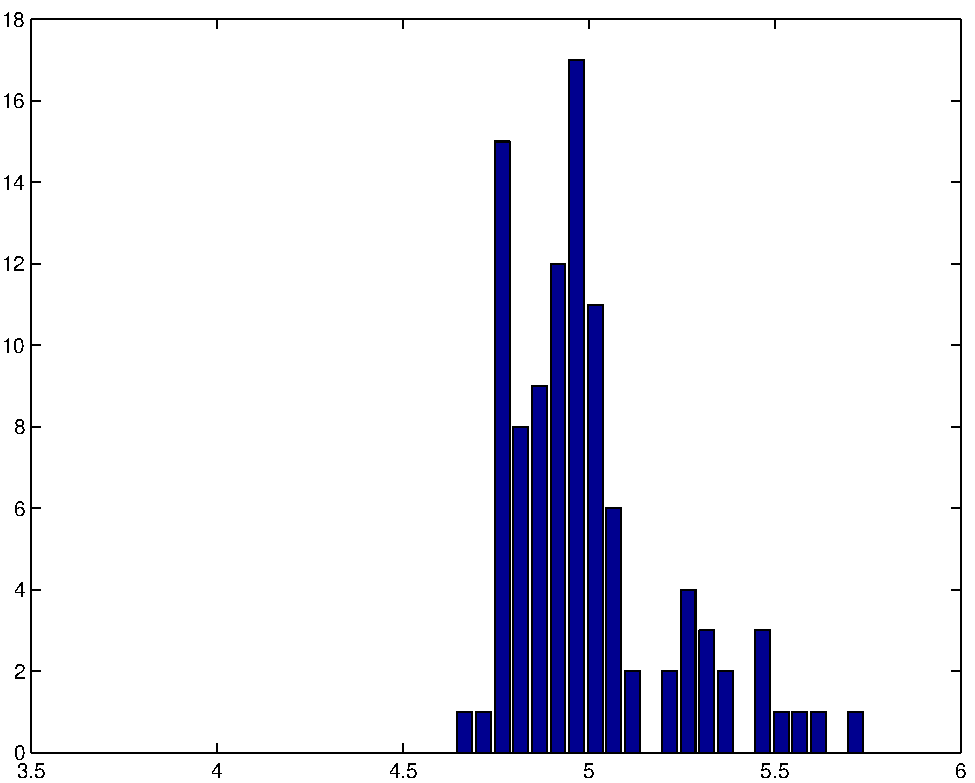
\includegraphics[width=5cm]{histojackreplicationsinflated}\\
\end{tabular}
\caption{Histograms of the bootstrap replications $\lbrace \hat{\theta}^{*}(b)\rbrace_{b\in \lbrace 1,\cdots,B=1000 \rbrace}$ (left), and the inflated jackknife replications $\lbrace \sqrt{n-1} (\hat{\theta}_{(i)}-\hat{\theta}_{(\cdot)})+ \hat{\theta}_{(\cdot)} \rbrace_{i\in \lbrace 1,\cdots,n=100 \rbrace}$ (right).}
\end{figure}
\end{exampleblock}

}
%%%%%%%%%%%%%%%%%%%%%%%%%%%%%%%%%%%%%%%%%%%%%%%%%%
\frame{
\frametitle{Relationship between jackknife and bootstrap}

\begin{itemize}
\item When $n$ is small, it is easier (faster) to compute the $n$ jackknife replications.

\

\item However the jackknife uses less information (less samples) than the bootstrap.

\

\item In fact, the jackknife is an  approximation to the bootstrap!   
\end{itemize}
}
%%%%%%%%%%%%%%%%%%%%%%%%%%%%%%%%%%%%%%%%%%%%%%%%%%%%
\frame
{
\frametitle{Relationship between jackknife and bootstrap}

\begin{itemize}
\item Considering a linear statistic : 
$$
\begin{array}{ll}
\hat{\theta}&=s(\mathbf{x})=\mu+\frac{1}{n} \sum_{i=1}^{n}\alpha(x_i)\\
&\\
&=\mu+\frac{1}{n} \sum_{i=1}^{n}\alpha_i\\
\end{array}
$$
\begin{exampleblock}{Mean $\hat{\theta}=\overline{x}$}
The mean is linear $\mu=0$ and $\alpha(x_i)=\alpha_i=x_i,\quad \forall i\in \lbrace 1,\cdot,n\rbrace$.
\end{exampleblock}
\item There is no loss of information in using the jackknife to compute the standard error (compared to the bootstrap) for a linear statistic. Indeed the knowledge of the $n$ jackknife replications $\lbrace \hat{\theta}_{(i)} \rbrace$, gives the value of $\hat{\theta}$ for any bootstrap data set. 
 
\item For non-linear statistics, the jackknife makes a linear approximation to the bootstrap  for the standard error. 

\end{itemize}

}
%%%%%%%%%%%%%%%%%%%%%%%%%%%%%%%%%%%%%%%%%%%%%%%%%%%%
\frame
{
\frametitle{Relationship between jackknife and bootstrap}


\begin{itemize}
\item Considering a quadratic  statistic
$$
\begin{array}{ll}
\hat{\theta}&=s(\mathbf{x})=\mu+\frac{1}{n} \sum_{i=1}^{n}\alpha(x_i)+\frac{1}{n^2} \beta(x_i,x_j)\\
\end{array}
$$
\begin{exampleblock}{Variance $\hat{\theta}=\hat{\sigma}^{2}$}
$\hat{\sigma}^{2}=\frac{1}{n}\sum_{i=1}^{n}(x_i-\overline{x})^2$ is a quadratic statistic.
\end{exampleblock}

\item Again the knowledge of the $n$ jackknife replications $\lbrace s(\hat{\theta}_{(i)}) \rbrace$, gives the value of $\hat{\theta}$ for any bootstrap data set. The jackknife and bootstrap estimates of the bias agree for quadratic statistics. 
\end{itemize}

}
%%%%%%%%%%%%%%%%%%%%%%%%%%%%%%%%%%%%%%%%%%%%%%%%%%%%
\frame
{
\frametitle{Relationship between jackknife and bootstrap}
\begin{exampleblock}{The Law school example: $\hat{\theta}=\widehat{\mathrm{corr}}(\mathbf{x},\mathbf{y})$.}
The correlation is a non linear statistic.
\begin{itemize}
\item From B=3200 bootstrap replications, $\hat{\mathrm{se}}_{B=3200}=0.132$. 
% $\mathbb{E}\lbrack\hat{\mathrm{se}}_{B=100}\rbrack=0.132$. 
%(and standard deviation $0.0117$).

\

\item From $n=15$ jackknife replications, $\hat{\mathrm{se}}_{jack}= 0.1425$.

\

\item Textbook formula: 
$\mathrm{se}_{\hat{f}}=(1-\widehat{\mathrm{corr}}^2)/\sqrt{n-3}=0.1147$
\end{itemize}
\end{exampleblock}

}
%%%%%%%%%%%%%%%%%%%%%%%%%%%%%%%%%%%%%%%%%%%%%%%%%%%%
\frame{
\frametitle{Failure of the jackknife}

The jackknife can fail if the estimate $\hat{\theta}$ is not smooth (i.e. a small change in the data can cause a large change in the statistic).
A simple non-smooth statistic is the median.
\begin{exampleblock}{On the mouse data}
Compute the jackknife replications of the median $\mathbf{x}_{Cont}=(10,27,31,40,46,50,52,104,146)$ (Control group data).
\begin{itemize}
\item  You should find 48,48,48,48,45,43,43,43,43 \footnote{The median of an even number of data points is the average of the middle 2 values.}. 

\

\item Three different values appears as  a consequence of a lack of smoothness of the median\footnote{the median is not a differentiable function of $x$.}. 
\end{itemize} 
\end{exampleblock}
}
%%%%%%%%%%%%%%%%%%%%%%%%%%%%%%%%%%%%%%%%%%%%%%%%%%%%
%\frame
%{
%\frametitle{Relationship between jackknife and bootstrap}
%
%\begin{table}[!h]
%\begin{tabular}{p{2cm}|p{2cm}|p{2cm}|p{2cm}|p{2cm}}
%$\hat{\theta}$ & linear & quadratic & non-linear (but smooth) & non-smooth\\
%\hline
%jackknife se &  agree with bootstrap  & linear approx. of bootstrap se &  
%linear approx. of bootstrap se & fails \\
% \hline
%jackknife bias & agree with bootstrap bias & agree with bootstrap bias & approx. of bootstrap & fails\\
%  \end{tabular}
%\end{table}
%}

%%%%%%%%%%%%%%%%%%%%%%%%%%%%%%%%%%%%%%%%%%%%%%%%%%%%
%\frame{
%\frametitle{Jackknife and Bootstrap}
%\begin{block}{}
%\begin{itemize}
%\item we can easily compute the whole $n$ jackknife samples when $n<100\ \mathrm{to}\ 200$. However the jackknife uses only limited information about the statistic $\hat{\theta}$.
%\item In fact, the jackknife  makes a \textit{linear}
%\footnote{if $F_1$, $F_2$ are two distributions, then $\theta=t(\lambda F_1+(1-\lambda) F_2)=\lambda t(F_1)+(1-\lambda) t(F_2)$.} 
%approximation to the bootstrap.
%\item Practically, accuracy of the jackknife estimate of se depends on how close $\hat{\theta}$ is to being a linear function of $\mathbf{x}$.
%\end{itemize}
%\end{block}
%}
%%%%%%%%%%%%%%%%%%%%%%%%%%%%%%%%%%%%%%%%%%%%%%%%%%%%
\frame
{
\frametitle{Delete-d Jackknife samples}
\begin{definition}
The \alert{delete-d Jackknife} subsamples are computed by leaving out $d$ observations from $\mathbf{x}$ at a time.   
\end{definition}

\begin{beamercolorbox}[wd=\linewidth, rounded=true,shadow=true]{postit}
\begin{itemize}
\item The dimension of the subsample is  $n-d$.
\item The number of possible subsamples now rises $\left(\begin{array}{c}n \\ d\end{array}\right)
=\frac{n!}{d!(n-d)!}$.
 \item  Choice: $\sqrt{n}< d< n$
\end{itemize}
\end{beamercolorbox}



}
%%%%%%%%%%%%%%%%%%%%%%%%%%%%%%%%%%%%%%%%%%%%%%%%%%%%
\frame{
\frametitle{Delete-d jackknife}

\begin{beamercolorbox}[wd=\linewidth, rounded=true,shadow=true]{postit}

\begin{enumerate}
\item Compute all $\left(\begin{array}{c}n \\ d\end{array}\right)$  d-jackknife subsamples $\mathbf{x}_{(1)}, \cdots,\mathbf{x}_{(n)}$ from $\mathbf{x}$.

\

\item Evaluate the jackknife replications $\hat{\theta}_{(i)}=s(\mathbf{x}_{(i)})$.

\

\item Estimation of the standard error (when $n=r\cdot d$):
$$
\widehat{\mathrm{se}}_{d-jack}=\left \lbrace \frac{r}{\left(\begin{array}{c}n \\ d\end{array}\right)} \sum_{i} (\hat{\theta}_{(i)} -\hat{\theta}(\cdot))^2 \right\rbrace^{1/2}
$$
where $\hat{\theta}(\cdot)=\frac{\sum_{i} \hat{\theta}_{(i)} }{\left(\begin{array}{c}n \\ d\end{array}\right)} $. 
\end{enumerate}



\end{beamercolorbox}
}

%%%%%%%%%%%%%%%%%%%%%%%%%%%%%%%%%%%%%%%%%%%%%%%%%%%%
\frame
{
\frametitle{Concluding remarks} 

\begin{itemize}
\item The inconsistency of the jackknife subsamples with non-smooth statistics can be fixed using  delete-d jackknife subsamples.

\

\item The subsamples (jackknife or delete-d jackknife) are actually samples (of smaller size) from the true distribution $f$ whereas resamples (bootstrap) are samples from  $\hat{f}$.  
%\item Distribution estimates based on subsampling are valid in a wider range of situations than their resampling (i.e. bootstrap) analogs, even in the cases where the statistics $s(\mathbf{x})$ is not asymptotically normal.
%\item However, they do not possess the property of higher-order accuracy mainly because of the subsampling size $m<n$.

\

%\item In practice, sampling \textit{with} or \textit{without} replacement from the original sample  $\mathbf{x}$ would  make no difference if $m$ is very small w.r.t. $n$ (i.e. $\frac{m}{\sqrt{n}}\rightarrow 0$).      
\end{itemize}
}
%%%%%%%%%%%%%%%%%%%%%%%%%%%%%%%%%%%%%%%%%%%%%%%%%%%%
\frame{
\frametitle{Summary}

\begin{itemize}
%\item Jackknife/ delete-d jackknife subsamples
\item Bias and standard error estimates have been introduced  using jackknife replications.

\

\item The Jackknife standard error estimate is a linear approximation of the bootstrap standard error.

\

\item The Jackknife bias estimate is a quadratic approximation of the bootstrap bias.

\


\item Using smaller subsamples (delete-d jackknife) can improve for non-smooth statistics  such as the median.
\end{itemize}
}
